%Building
\documentclass[11pt]{article}

\usepackage[english]{babel}
\usepackage[margin=1in]{geometry}
\usepackage[colorlinks=true, allcolors=blue]{hyperref}

% Math/Greek packages
\usepackage{amssymb, amsmath, amsthm, mathtools, esint} 
\usepackage{algorithm, algorithmic}
\usepackage{upgreek}
\usepackage{physics}

% Graphics/Presentation packages
\usepackage{graphicx}
\usepackage{multirow, subcaption, cleveref}
\usepackage{tabulary, enumitem}
\usepackage{cancel}

%replace "ref" with "cref", "Cref", "crefrange"

% Misc packages
\renewcommand\qedsymbol{\textit{``Quack"}} %change the QED symbol to ``Quack" for the inside joke of Quantum Entangled Ducks

% defining where the images are
\graphicspath{ {../ESOF 322 Project (drive copy)/} }


\usepackage{fontspec}
% Use this line to change the font of your file. If you have the Open Dyslexic v. 1 downloaded (bold-italic- bolditalics included), you can use this line. This font addresses Dyslexic people. 
%\setmainfont{OpenDyslexic}
% Use this line to change the font of your file. If you have the Atkinson Hyperlegible downloaded (bold-italic- bolditalics included), you can use this line. This font addresses sight-impaired peoples
%\setmainfont{Atkinson Hyperlegible}

\begin{document}

\title{ESOF 322: Project 1 - Cold Case Database}
\author{Jacob Coleman, William Jardee, Fletcher Philips, Megan Steinmasel}
\maketitle


%%TO-DO
\begin{figure}[!ht]
\centering
\textbf{Author: Megan Steinmasel}
\vspace{1em}

	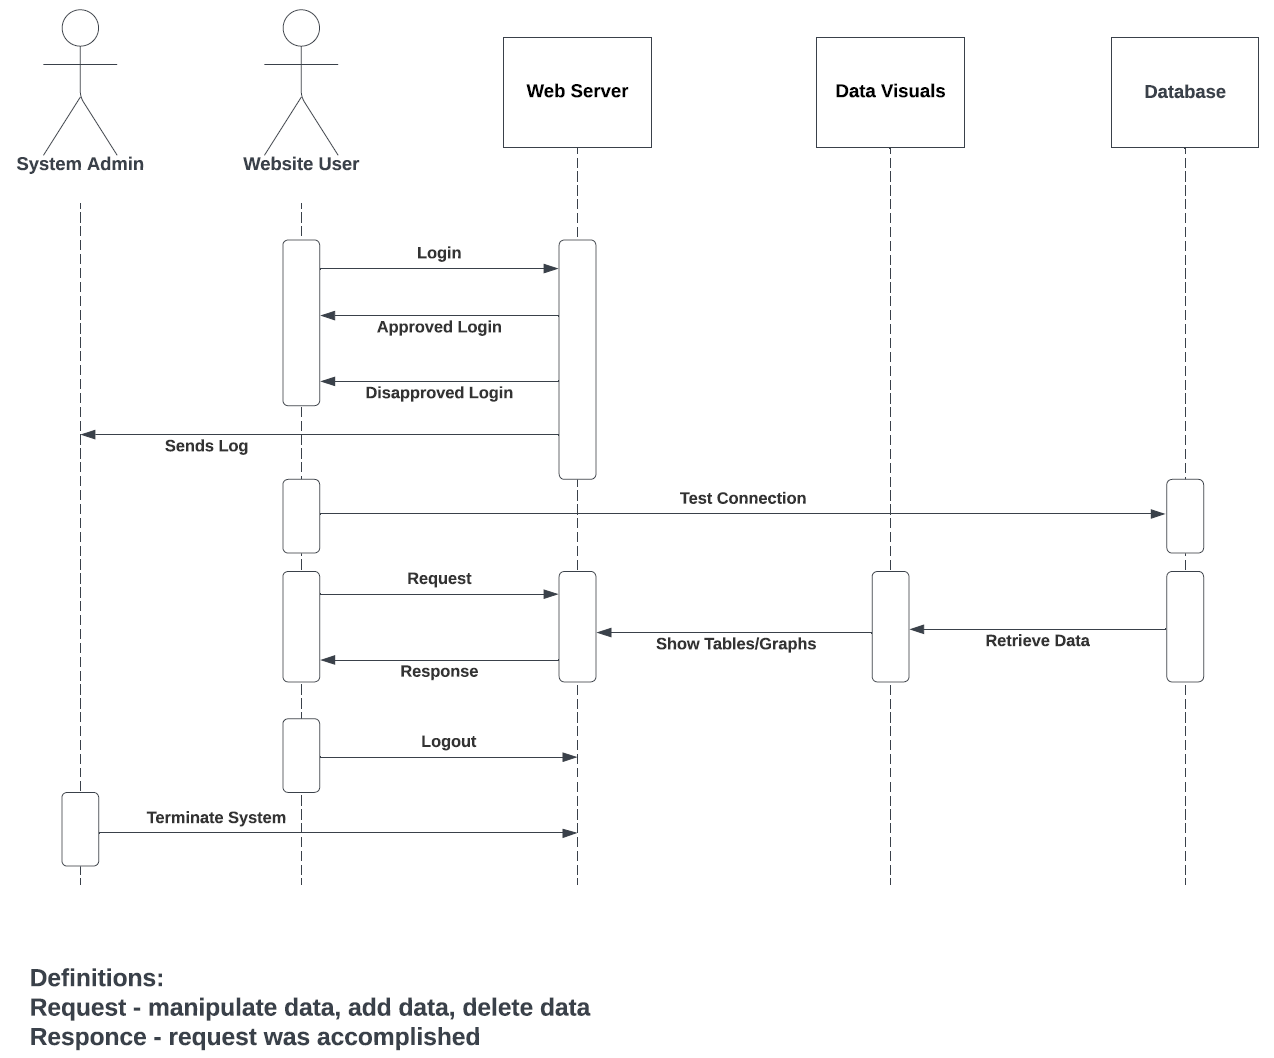
\includegraphics[width=.85\textwidth]{./project2-Diagrams/ccsequence.png}\\
	\caption{Sequence Diagram for Cold-Cases Database system.}
	\label{fig:ccSequence}
\end{figure}

\begin{figure}[!ht]
\centering
\textbf{Author: Fletcher Philips}
\vspace{1em}

	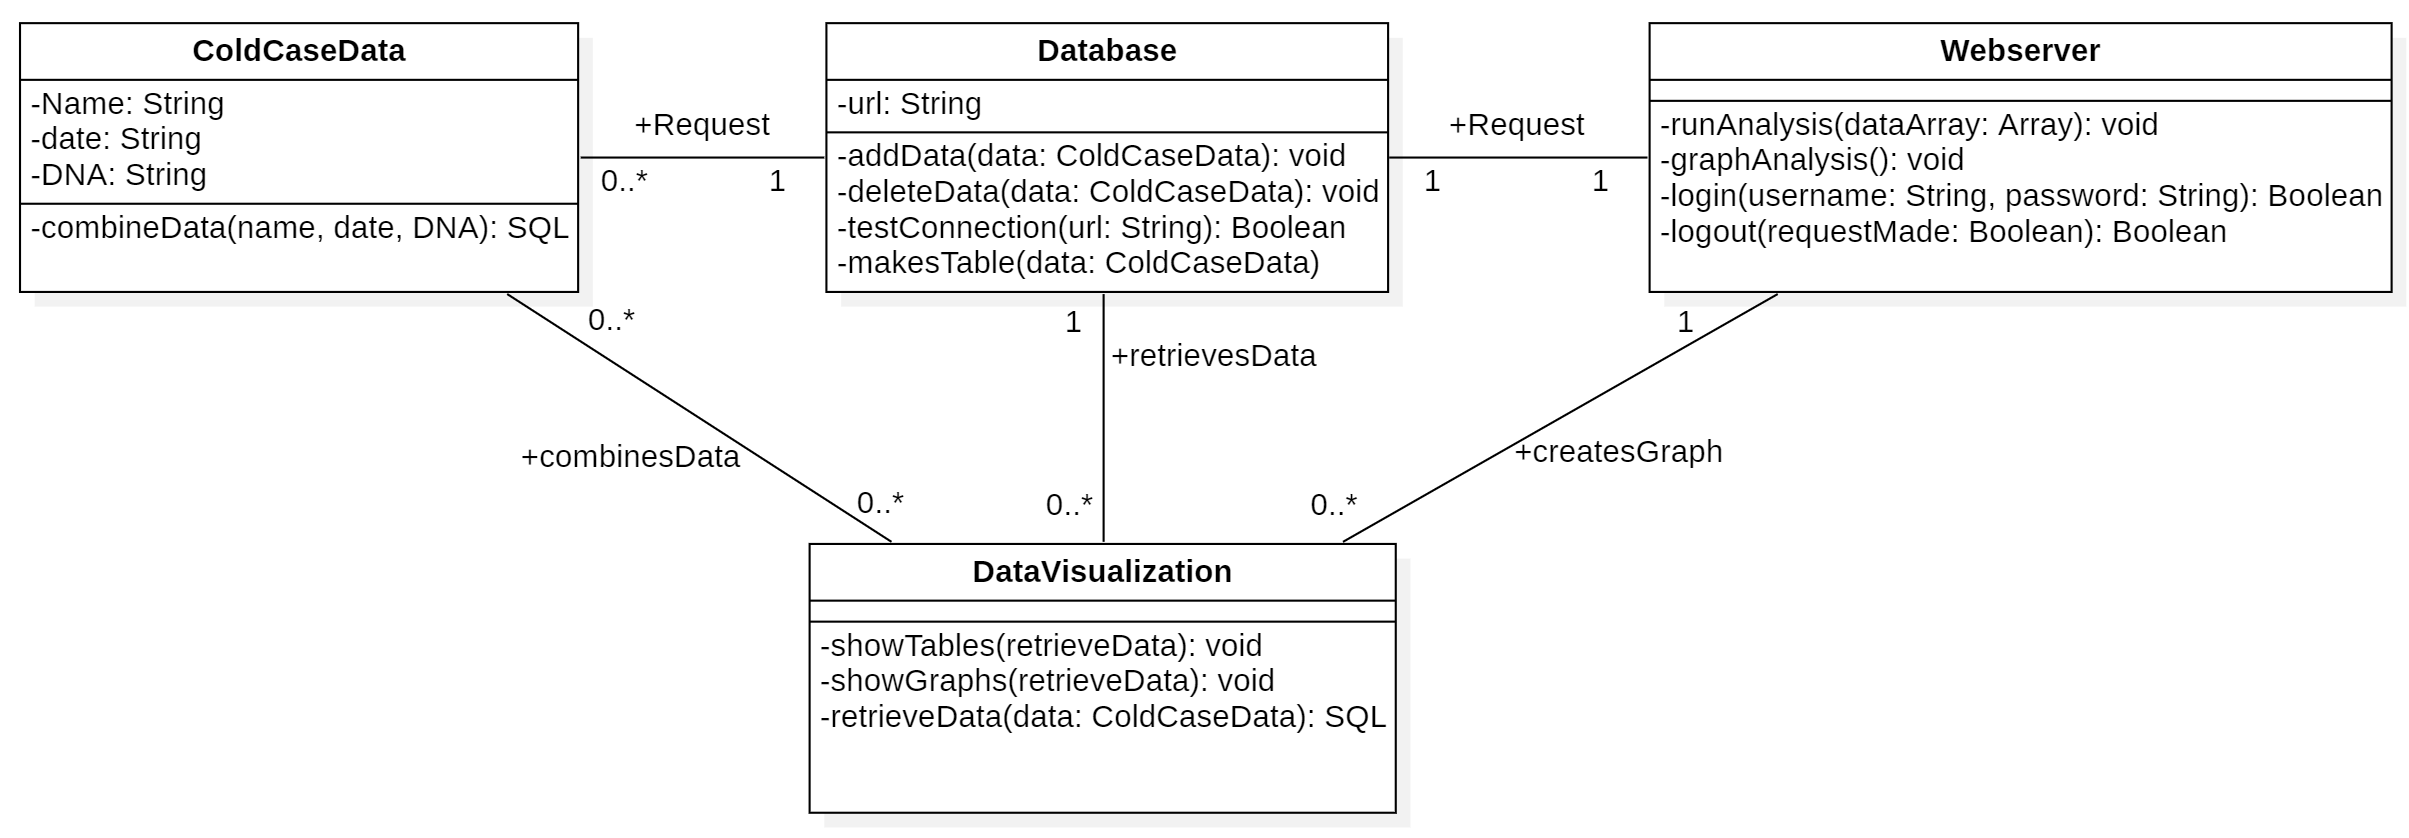
\includegraphics[width=.95\textwidth]{./project2-Diagrams/project2ClassDiagram.png}\\
	\caption{Class diagram for the Cold-Cases Database system.}
	\label{fig:classDiagram}
\end{figure}

\end{document}
